% =====================================================================
%  AL-FAJAR RESOURCES — COMPANY PROFILE (distribution partnership)
%  -------------------------------------------------------------------
%  Compile:   tectonic al-fajar-company-profile.tex
%             (or upload to Overleaf — all packages are standard)
%
%  How to edit:
%    1. Company facts (name, contact, prepared-for) live in one block
%       near the bottom of the preamble — change them once.
%    2. Every yellow [BOX] in the PDF is an unfilled fact. Search the
%       source for \todo{ and replace each with the real text.
%    3. Colours are defined in the "Colour palette" block — edit once.
%    4. Body text: sections below are clearly separated by comments.
%    5. The operations chart is drawn with TikZ — instructions are
%       commented inside it.
% =====================================================================
\documentclass[11pt,letterpaper]{article}

%% ---------------------------- Fonts ---------------------------------
\usepackage[T1]{fontenc}
\usepackage[utf8]{inputenc}
\usepackage{tgtermes}                 % body — Times-like serif
\usepackage{tgheros}                  % headings — Helvetica-like sans
\usepackage{amssymb}
\hyphenation{Al-Fajar Resources}       % never break inside the brand name

%% ---------------------------- Layout --------------------------------
\usepackage[margin=1in, top=0.95in, bottom=0.95in]{geometry}
\usepackage{microtype}
\usepackage{soul}                    % breakable yellow highlight for \todo
\hyphenpenalty=10000 \exhyphenpenalty=10000   % never hyphenate
\usepackage{graphicx}
% Image locations — logo in app/public/, cover image next to this file
\graphicspath{{app/public/}{./}}
\emergencystretch 1.5em
\setlength{\parindent}{0pt}
\setlength{\parskip}{0.6em}

%% ------------------------- Colour palette ---------------------------
\usepackage{xcolor}
\definecolor{corpblue}{RGB}{31,73,125}      % primary — deep corporate blue
\definecolor{gold}{RGB}{175,141,44}         % accent — muted gold
\definecolor{lightbox}{RGB}{241,245,250}    % light fill for boxes
\definecolor{bodytext}{RGB}{40,40,40}       % body text
\definecolor{rulegray}{RGB}{176,176,176}    % thin outline for item boxes

%% ---------------------------- Headings ------------------------------
\usepackage{titlesec}
\usepackage{needspace}                 % keep headings with following content
% never let a section heading (and its rule) strand at a page bottom
\let\OmpOldSection\section
\renewcommand{\section}{\needspace{5\baselineskip}\OmpOldSection}
\titleformat{\section}
  {\sffamily\Large\bfseries\color{corpblue}}
  {\thesection.}
  {0.6em}
  {}
  [\vspace{0.15em}{\color{gold}\titlerule[0.7pt]}]
\titlespacing*{\section}{0pt}{2.2em}{1.0em}
% sub-headings (used inside section 7)
\let\OmpOldSubsection\subsection
\renewcommand{\subsection}{\needspace{4\baselineskip}\OmpOldSubsection}
\titleformat{\subsection}
  {\sffamily\large\bfseries\color{corpblue}}
  {}
  {0pt}
  {}
\titlespacing*{\subsection}{0pt}{1.2em}{0.3em}

%% ----------------------------- Lists --------------------------------
\usepackage{enumitem}
\setlist[itemize,1]{%
  label=\textcolor{gold}{\raisebox{0.28em}{\tiny$\blacksquare$}},
  leftmargin=1.6em, itemsep=0.35em, topsep=0.35em
}
\setlist[enumerate,1]{%
  label=\textcolor{gold}{\sffamily\bfseries\arabic*.},
  leftmargin=1.8em, itemsep=0.35em, topsep=0.35em
}

%% ----------------------------- Tables -------------------------------
\usepackage{booktabs}
\usepackage{tabularx}
\usepackage{colortbl}                 % colored table rules
% Two-column fact table (used by sections 1 and 10). Rows: Label & Value \\
% with \midrule between rows; the last row has no \midrule after it.
\newenvironment{facttable}{%
  \arrayrulecolor{corpblue}%
  \renewcommand{\arraystretch}{1.8}%
  \tabularx{\linewidth}{@{}>{\sffamily\bfseries\color{corpblue}}m{4.8cm} >{\raggedright\arraybackslash}X@{}}%
  \toprule}{%
  \bottomrule
  \endtabularx}

%% --------------------------- Boxes / chart --------------------------
\usepackage{tcolorbox}
\usepackage{tikz}


%% ------------------------ Header / footer ---------------------------
\usepackage{fancyhdr}
\pagestyle{fancy}
\fancyhf{}
\fancyfoot[L]{\sffamily\footnotesize\color{corpblue}\CompanyName{} \textbullet\ Company Profile}
\fancyfoot[R]{\sffamily\footnotesize\color{corpblue}Page \thepage}
\renewcommand{\headrulewidth}{0pt}

%% --------------------------- Hyperlinks -----------------------------
\usepackage[colorlinks=true, allcolors=corpblue,
  pdftitle={Al-Fajar Resources - Company Profile},
  pdfauthor={Al-Fajar Resources}]{hyperref}

%% =====================================================================
%%  EDIT ME — company facts (used throughout the document)
%% =====================================================================
% Highlights an unfilled fact. Replace each \todo{...} with the real text.
\sethlcolor{yellow}
\newcommand{\todo}[1]{{\color{black}\bfseries\hl{[#1]}}}

\newcommand{\CompanyName}{Al-Fajar Resources}
\newcommand{\Tagline}{Powering Performance through Global Lubricant Solutions \& Trade Excellence} % kept, currently unused
\newcommand{\CompanyBusiness}{Lubricants trading, import, and distribution}
\newcommand{\PreparedFor}{ENEOS Corporation}
\newcommand{\ContactName}{Mr.~Sajid Javed}
\newcommand{\ContactEmail}{Sajid.combine@gmail.com}
\newcommand{\ContactMobile}{(+92) 300 8432850}
\newcommand{\ContactLandline}{(+92) 423 7722676}
\newcommand{\ContactAddress}{Plot No.4, Oil Lane, Badami Bagh, Lahore, Pakistan}

\begin{document}
\raggedright                            % left-aligned body, no hyphenation

%% ================================ COVER ==============================
% No footer, roman numerals so the first inner page can restart at 1.
\pagenumbering{roman}
\thispagestyle{empty}
\null
\begin{tikzpicture}[remember picture, overlay]
  % full-bleed background (scaled to page width, centre-cropped)
  \clip (current page.south west) rectangle (current page.north east);
  \node at (current page.center)
    {\includegraphics[width=\paperwidth]{cover.png}};
  % navy overlay, lower half, 55 % opacity
  \fill[corpblue, opacity=0.55]
    (current page.south west) rectangle (current page.east);
  % logo on a white circular backing (logo is navy, sky is navy-ish)
  \fill[white] ([yshift=-4.6cm]current page.north) circle (1.75cm);
  \node at ([yshift=-4.6cm]current page.north)
    {\includegraphics[height=3cm]{logo-circle.png}};
  % title block
  \node[text width=0.8\paperwidth, align=center, text=white]
    at ([yshift=7.2cm]current page.south) {%
    {\sffamily\bfseries\fontsize{36}{42}\selectfont Company Profile}\\[0.6em]
    {\sffamily\Large Distribution Partnership Proposal}\\[1.0em]
    {\color{gold}\rule{0.3\linewidth}{1pt}}\\[1.0em]
    {\sffamily\large Prepared for \PreparedFor}\\[0.4em]
    {\sffamily\large\bfseries \CompanyName}\\[0.4em]
    {\sffamily\large October 2026}};
  % confidentiality line
  \node[anchor=south, text=white, font=\sffamily\footnotesize]
    at ([yshift=1.2cm]current page.south)
    {Confidential. Prepared for \PreparedFor.};
\end{tikzpicture}
\clearpage
\pagenumbering{arabic}                  % page 1 = first inner page

%% ========================= COMPANY AT A GLANCE =======================
\section{Company at a Glance}

\begin{facttable}
  Legal Name & \CompanyName \\
  \midrule
  Business & \CompanyBusiness \\
  \midrule
  Established & 2000 \\
  \midrule
  Headquarters & Lahore, Pakistan \\
  \midrule
  Registration & Lahore Chamber of Commerce \& Industry, No. 91666-A; Tax ID: 0201228-6 \\
  \midrule
  Territory of Interest & South Asia \& Middle East \\
  \midrule
  % Customer Segments & \todo{e.g., industrial plants, transport fleets, automotive workshops, retail dealers} \\
  % \midrule
  % Storage Capacity & \todo{XX} square metres in \todo{LOCATION} \\
  % \midrule
  Team & 13 staff across sales, logistics, and administration \\
  \midrule
  Other Brands Handled & Buckman \\
  \midrule
  Proposed Role & Authorized distributor of ENEOS lubricants \\
\end{facttable}

%% ================================ WHO WE ARE =========================
\section{Who We Are}

\textbf{\CompanyName} is a lubricants trading and distribution company based in
Lahore, Pakistan. We import, store, and distribute lubricants and related
products to industrial, automotive, and commercial markets.

We would like to represent ENEOS as an authorized distributor.
Our approach is simple: sell with discipline, deliver on
time, protect the brand, and report openly to our principal. We are looking
for a long-term relationship, not a one-time transaction.

%% ============================ OUR COMMITMENT =========================
\section{Our Commitment}

\begin{tcolorbox}[colback=lightbox, colframe=corpblue, boxrule=0.6pt,
                  arc=1.5pt, left=1.2em, right=1.2em, top=0.7em, bottom=0.7em]
  {\sffamily\bfseries\color{corpblue}VISION}\\[0.3em]
  % To be a trusted, long-term distribution partner for leading lubricant
  % manufacturers in \todo{TERRITORY}.
  To be the premier global trade partner in high-performance lubricants and
  petroleum products, recognized for operational integrity, seamless
  logistics, and exceptional client satisfaction.

  \medskip
  {\sffamily\bfseries\color{corpblue}MISSION}\\[0.3em]
  % To deliver quality lubricants to our customers reliably and transparently,
  % while protecting the reputation of the brands we represent.
  To deliver superior lubrication solutions through a global trade network,
  empowering industries with high-efficiency products, transparent
  operations, and sustainable practices.
\end{tcolorbox}

%% ============================ CORE OPERATIONS ========================
\needspace{10cm}                        % heading + intro + chart stay together
\section{Core Operations}

Our operations are organised into three functions, each supporting the next.

\begin{center}
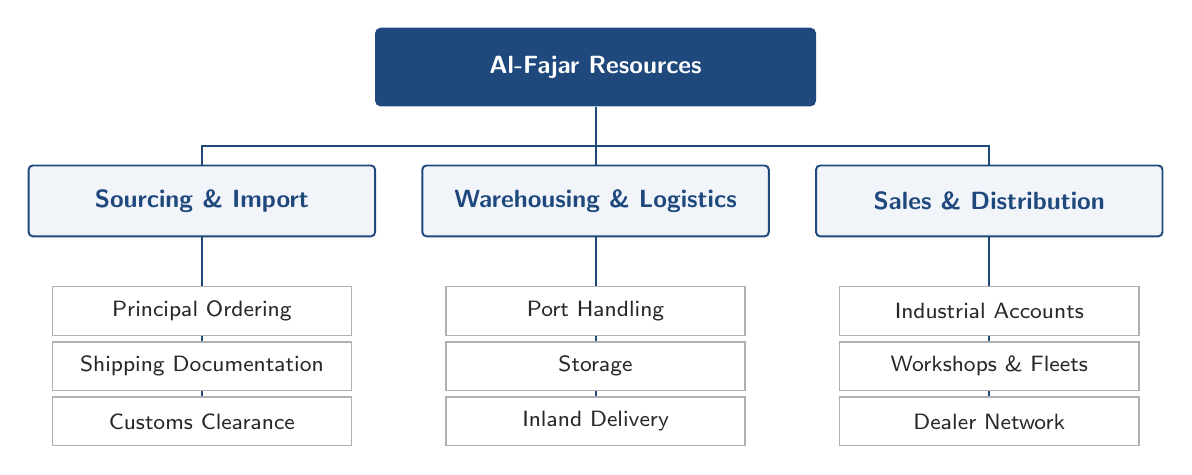
\begin{tikzpicture}[
  font=\sffamily,
  % --- chart style: edit visual look here -----------------------------
  topbox/.style={fill=corpblue, text=white, font=\sffamily\bfseries\small,
                 rounded corners=2pt, minimum width=5.6cm, minimum height=1.0cm,
                 align=center},
  branch/.style={fill=lightbox, draw=corpblue, line width=0.7pt,
                 text=corpblue, font=\sffamily\bfseries\small,
                 rounded corners=1.5pt, minimum width=4.4cm, minimum height=0.9cm,
                 align=center},
  item/.style={fill=white, draw=rulegray, line width=0.5pt, text=bodytext,
               font=\sffamily\footnotesize, minimum width=3.8cm,
               minimum height=0.62cm, align=center},
  conn/.style={corpblue, line width=0.7pt},
  % ---------------------------------------------------------------------
]
  % Tier 1 — company (edit label only)
  \node[topbox] (top) at (0,0) {\CompanyName};

  % Tier 2 — functions (to add one, copy a node + its 3 items and shift x)
  \node[branch] (b1) at (-5,-1.7) {Sourcing \& Import};
  \node[branch] (b2) at (0,-1.7)  {Warehousing \& Logistics};
  \node[branch] (b3) at (5,-1.7)  {Sales \& Distribution};

  % Tier 3 — function details
  \node[item] (a1) at (-5,-3.1) {Principal Ordering};
  \node[item] (a2) at (-5,-3.8) {Shipping Documentation};
  \node[item] (a3) at (-5,-4.5) {Customs Clearance};

  \node[item] (c1) at (0,-3.1)  {Port Handling};
  \node[item] (c2) at (0,-3.8)  {Storage};
  \node[item] (c3) at (0,-4.5)  {Inland Delivery};

  \node[item] (d1) at (5,-3.1)  {Industrial Accounts};
  \node[item] (d2) at (5,-3.8)  {Workshops \& Fleets};
  \node[item] (d3) at (5,-4.5)  {Dealer Network};

  % Connectors
  \draw[conn] (top.south) -- (0,-1.2);
  \draw[conn] (0,-1) -| (b1.north);
  \draw[conn] (0,-1) -| (b2.north);
  \draw[conn] (0,-1) -| (b3.north);

  \draw[conn] (b1.south) -- (a1.north);
  \draw[conn] (a1.south) -- (a2.north);
  \draw[conn] (a2.south) -- (a3.north);
  \draw[conn] (b2.south) -- (c1.north);
  \draw[conn] (c1.south) -- (c2.north);
  \draw[conn] (c2.south) -- (c3.north);
  \draw[conn] (b3.south) -- (d1.north);
  \draw[conn] (d1.south) -- (d2.north);
  \draw[conn] (d2.south) -- (d3.north);
\end{tikzpicture}
\end{center}

%% ================= WHAT WE BRING TO THE PARTNERSHIP ==================
\section{What We Bring to the Partnership}

\begin{itemize}
  \item \textbf{Global Supplier Network:} Direct access to tier-1 refineries
        and global lubricant formulators.
  \item \textbf{End-to-End Trade Solutions:} From factory floor sourcing to
        final destination customs clearance.
  \item \textbf{Customized Blending \& Sourcing:} Capability to source
        specialized fluid formulations tailored to specific climate and
        machinery demands.
  \item \textbf{Competitive Market Pricing:} Bulk purchasing power leveraged
        to offer maximum profitability to regional distributors and industrial
        end-users.
\end{itemize}

%% ============================ SUPPLY & LOGISTICS =====================
\section{Supply \& Logistics}

Reliable delivery is central to how we serve customers. Our logistics function
covers the full path from port of arrival to the customer's site.

\begin{itemize}
  \item \textbf{Import Operations:} Management of shipping documents and
        coordination with freight forwarders and shipping lines.
  \item \textbf{Customs Clearance:} Customs declarations, duty and tax
        payments, and regulatory filings in \todo{COUNTRY}.
  \item \textbf{Port Handling \& Inland Transport:} Offloading, container
        handling, and onward transport to our storage facility and customer
        sites.
  \item \textbf{Warehousing:} \todo{XX} square metres of storage in
        \todo{LOCATION} for packaged lubricants,
        \todo{DESCRIBE CONDITIONS, e.g., covered, dry, organised by batch}.
  \item \textbf{Packaging Formats:} Drums, pails, and IBC totes, with bulk
        formats where required.
  \item \textbf{Delivery:} Door-to-door delivery to customers in
        \todo{REGIONS}.
\end{itemize}

%% ================================ HOW WE WORK ========================
\section{How We Work}

\begin{enumerate}
  \item \textbf{Forecasting:} We share a rolling \todo{quarterly} demand
        forecast with ENEOS so supply can be planned ahead.
  \item \textbf{Ordering:} Orders are placed by purchase order, with payment
        under the agreed terms.
  \item \textbf{Shipping:} We coordinate booking, documentation, and shipment
        tracking with ENEOS and the freight forwarder.
  \item \textbf{Clearance and Receipt:} We handle customs clearance and
        inspect each delivery on arrival.
  \item \textbf{Storage and Delivery:} Products are stored at
        \todo{WAREHOUSE} and delivered to customers against confirmed orders.
  \item \textbf{Reporting:} We report sales, stock levels, and customer
        feedback to ENEOS \todo{monthly}.
\end{enumerate}

\subsection*{Product Integrity}

We store and handle products according to the manufacturer's guidelines. Batch
numbers are recorded on receipt and on delivery, so any product can be traced
to its shipment. We do not buy or sell products from unauthorized sources.

\subsection*{Compliance and Ethics}

We comply with the import, tax, and trade laws of \todo{COUNTRY}. We are
committed to ethical business practice and will follow ENEOS's compliance and
anti-corruption requirements.

%% ======================= OTHER TRADING ACTIVITIES ====================
\section{Other Trading Activities}

Alongside distribution, \CompanyName{} trades in other petroleum products,
including Group I, II, and III base oils and lubricant additive packages,
supplied in drums, IBCs, flexi tanks, and ISO tanks.
\todo{These activities will not conflict with our ENEOS distribution. We are willing to discuss exclusivity for ENEOS in the agreed territory.}

%% ========================= SUPPORTING DOCUMENTS ======================
% \section{Supporting Documents}

% The following documents are available on request:

% \begin{itemize}
%   \item Certificate of incorporation or business registration
%   \item Tax registration
%   \item Import and customs registrations
%   \item Bank reference letter
%   \item Warehouse details and photographs
%   \item Customer references
% \end{itemize}

%% ================================ CONTACT ============================
\needspace{9cm}                         % heading + table stay together
\section{Contact}

\begin{facttable}
  Company Name & \CompanyName \\
  \midrule
  Contact Person & \ContactName, CEO \\
  \midrule
  Email & \href{mailto:\ContactEmail}{\texttt{\ContactEmail}} \\
  \midrule
  Mobile & \ContactMobile \\
  \midrule
  Telephone & \ContactLandline \\
  \midrule
  Address & \ContactAddress \\
  \midrule
  Website & alfajarresources.netlify.app \\
\end{facttable}

\end{document}
